\graphicspath{{fig/introduction/}}

\chapter{Introduction}
\label{cha:introduction}

\section{Motivation}
\label{sec:motivation}

Many of us have been struck by the inherent beauty of animals moving collectively;
starlings gathering in huge numbers at dusk to perform the most mesmerising of ballets,
the entire flock moving as if some fluid object (\cref{fig:murmuration}); fish forming
tight milling structures in defence against predation (\cref{fig:milling}), changing
direction in the blink of an eye and with a flash of silver.  Collective motion, broadly
defined as the formation of macro-level structures from the interactions of individuals
\parencite{camazine03}, has been observed over many different length scales, and has been
exhibited by many different species \parencite{allee31}. But through all its variations
and incantations, the one thing that remains constant is the phenomenon's ability to
capture the attention and wonder of the observer.

\begin{figure}[tb]
    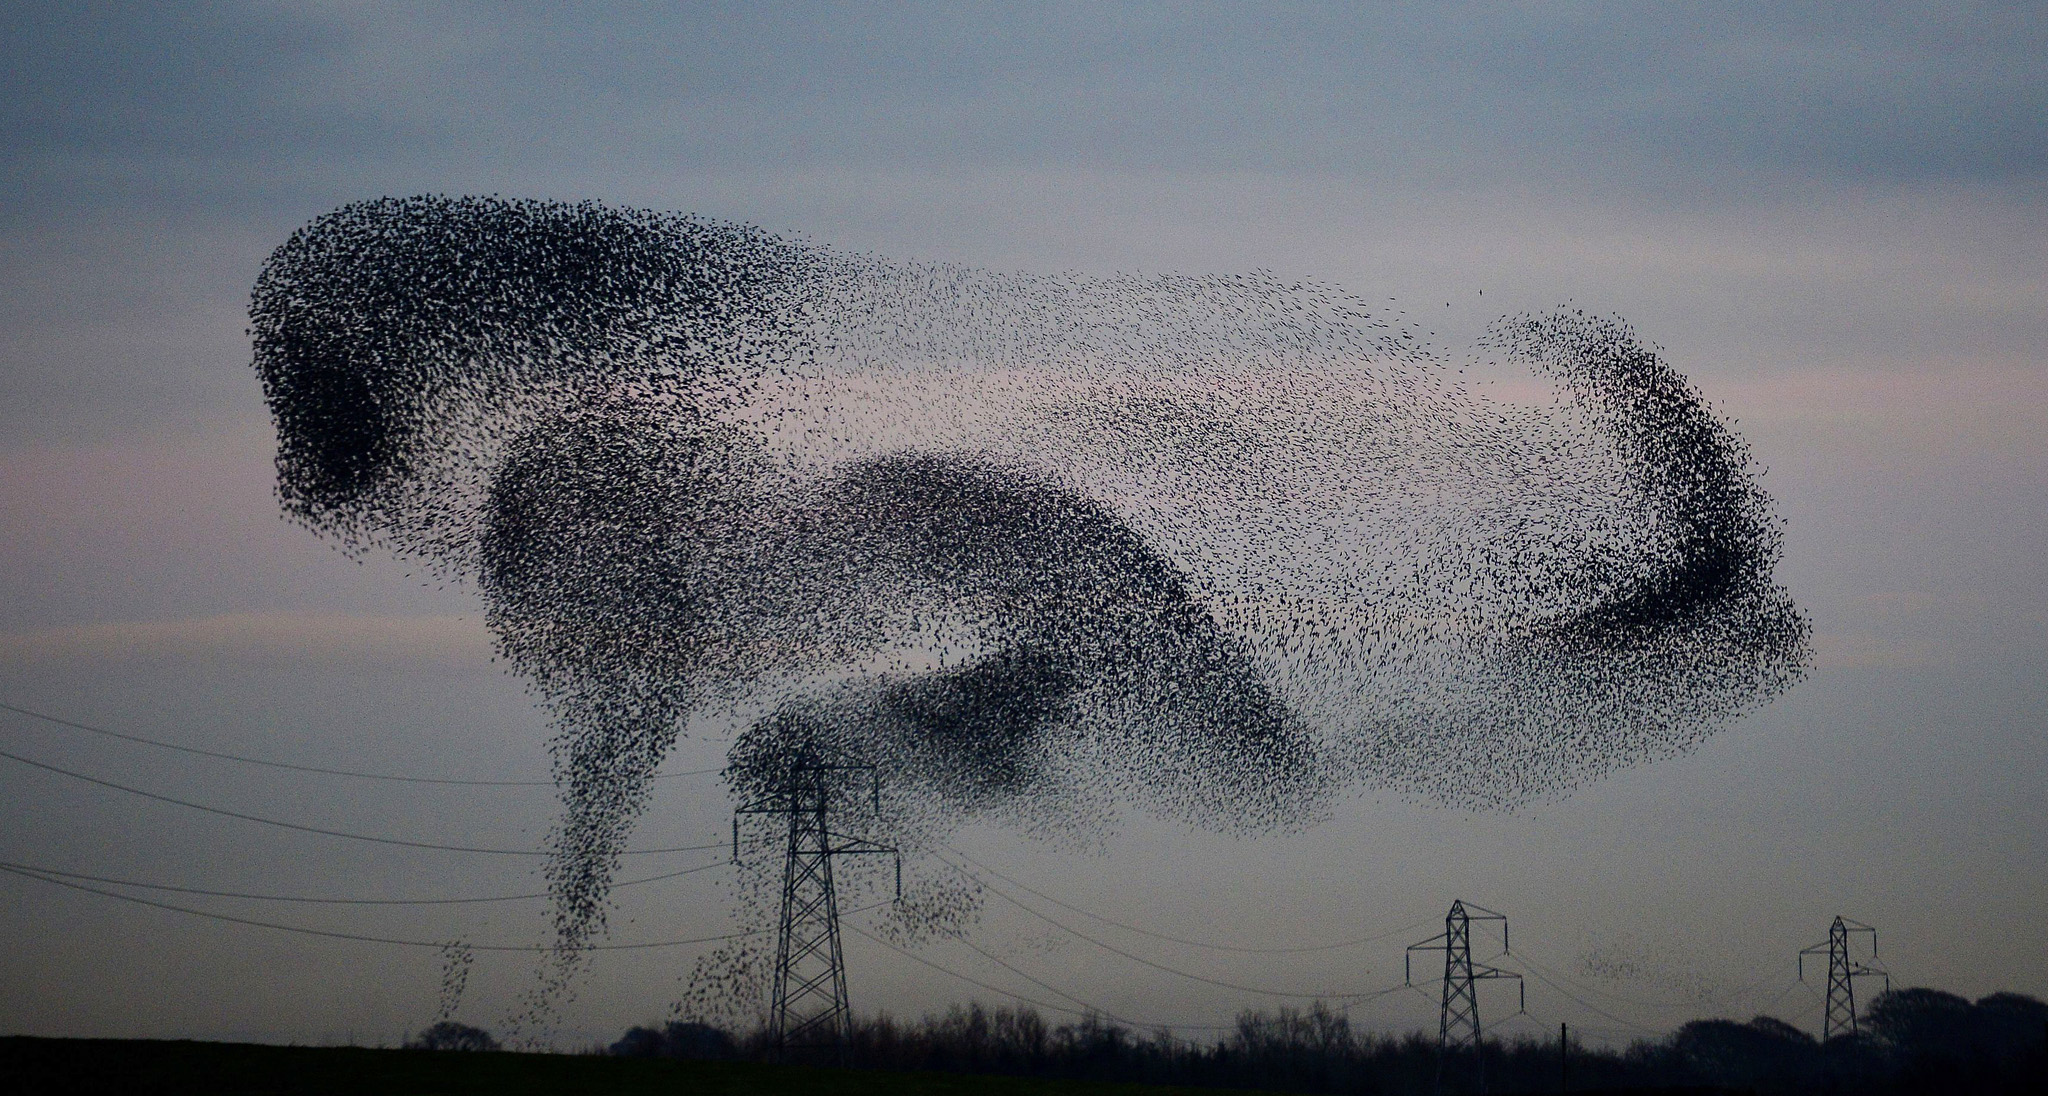
\includegraphics[width=\textwidth]{murmuration.jpg}
    \caption{A particularly startling example of a starling murmuration, captured near
        Gretna in the Scottish Borders. Photograph: Owen Humphreys/PA.}
    \label{fig:murmuration}
\end{figure}

Through captured imaginations, and over the years, collective behaviour has become a
thriving topic of multidisciplinary research, holding captive the minds of physicists,
biologists, mathematicians, and many others of the scientific persuasion. Though our
understanding has evolved significantly from early suggestions that collective behaviour
results from thought-transference and telepathy between individuals \parencite{selous31},
there is still so much that remains unknown.

In many cases, the \emph{why} of collective behaviour is broadly understood. From an
evolutionary standpoint, we can reason about the benefits which collective behaviour
brings to the individuals involved. For example, it is known that aggregation can provide
an effective defence against predation \parencite{landeau86}, and that both foraging and
migration can benefit from the knowledge of the collective \parencite{simmons04}.

Despite this, much less about the \emph{how} of collective behaviour is known. The
mechanisms which lead to the formation and maintenance of aggregations remain more
elusive, and are a topic of much interest. The hope is that the study of mathematical
models of flocking, and the comparison of these models with real flocking events, will
shed light on the mechanics which underlie these phenomena. In recent years modern
computing power has made the process of simulating these models relatively pain-free,
however, a lack of quality data detailing real flocking events has made the comparison
between model and data difficult.

Previously, much work has been invested in developing the theoretical models which seek to
explain emergent behaviour by interactions at an individual level. Such models have shown
that individual interactions are sufficient to produce group-level structures
\parencite{aoki82}. Many different simulations, implementing disparate interaction rules,
are able to produce behaviour reminiscent of real flocking systems. However, these models
have largely only been verified with comparison to empirical observation at a qualitative
level, and thorough quantitative comparison between field data and theory has been
lacking. This lack of quantitative comparison between model and data can largely be
attributed to the scarcity of empirical data.

However, in recent years technological and methodological advances have made it possible
to capture the movements of large groups of animal aggregates \parencite{ballerini08}.
With this data, it is only now that we are in a position to make robust comparison between
model prediction and real-world observation.

Using recently collected data, this thesis seeks to compare newly available data of
flocking events and theoretical models. The intention is to fit multiple different models
to the same dataset. With this we will be in a position to consider which of the fitted
models best describes the observed data.

\begin{figure}[tb]
    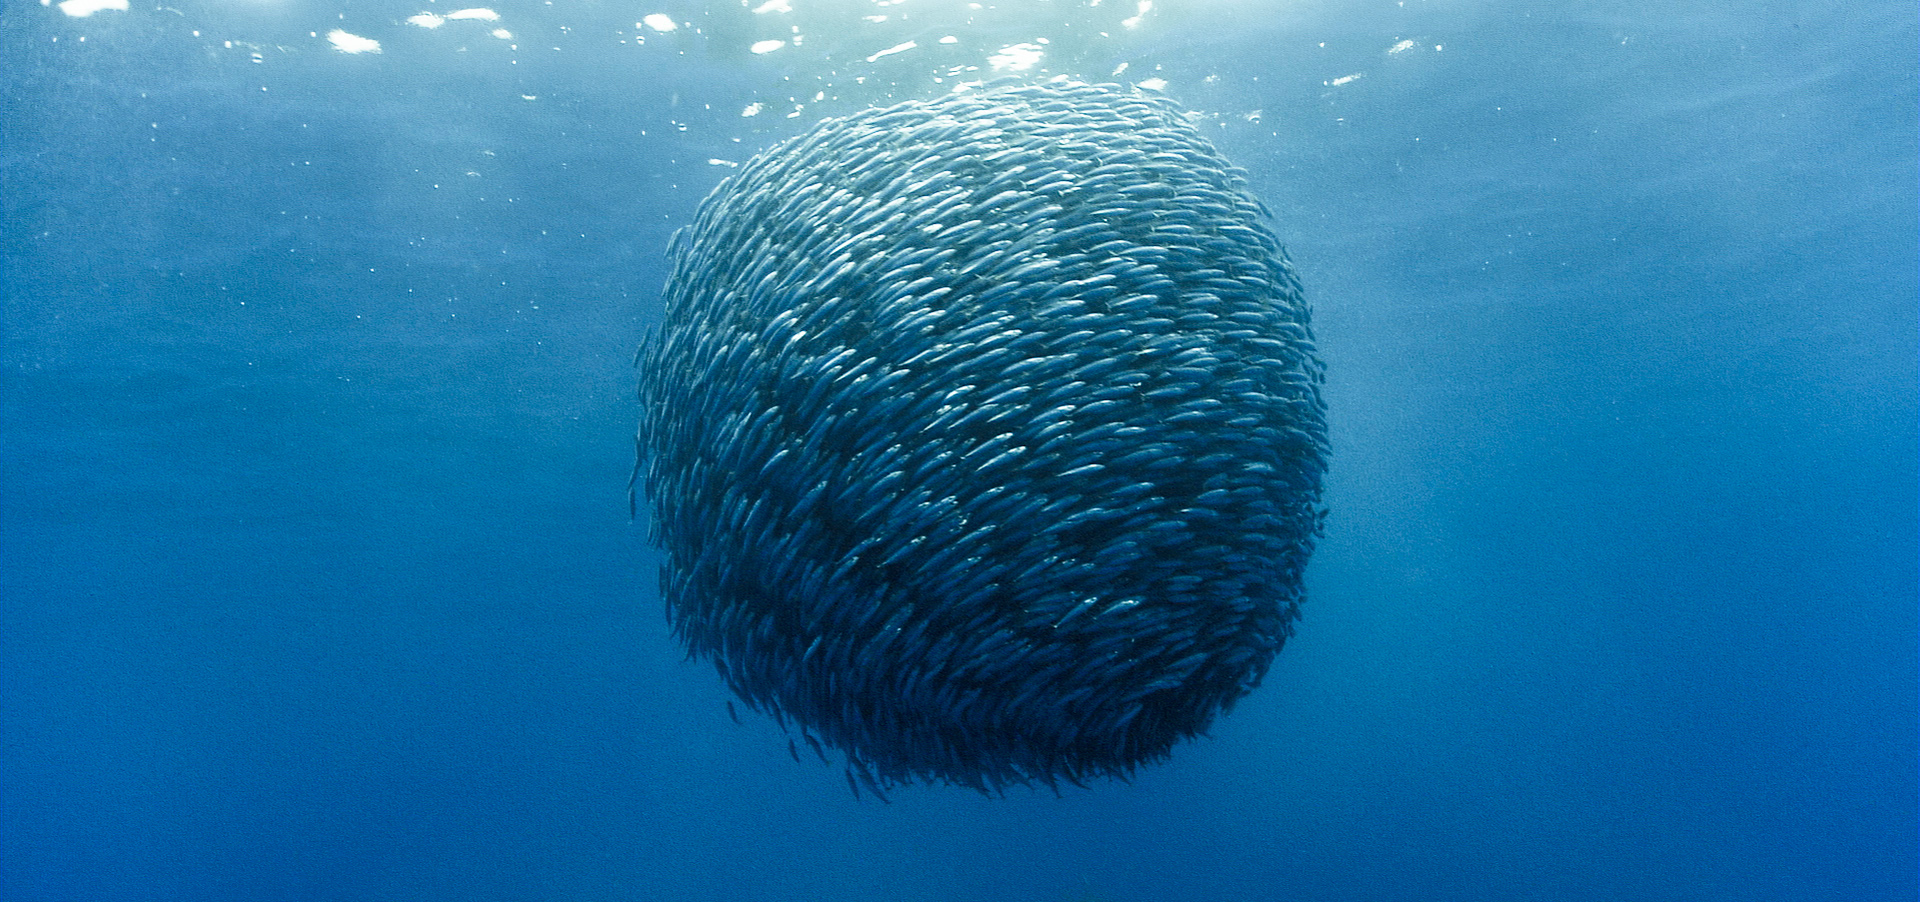
\includegraphics[width=\textwidth]{milling.jpg}
    \caption{Mackerel form a milling structure as a defence against predation.}
    \label{fig:milling}
\end{figure}

\section{Thesis overview}
\label{sec:overview_of_thesis}

We get the ball rolling in \cref{cha:lit_review} by giving the reader a
review of the literature surrounding collective behaviour. Important results and ideas of
the field are introduced and discussed. After relaying the main results from the
literature we discuss open problems and the future of research in the field.

Bayesian statistics will be introduced to the reader in \cref{cha:bayes_intro}. Important
results, techniques and algorithms from the subject will be outlined as well as any
problems that a Bayesian practitioner may encounter, and how they may address these problems.

Proceeding onwards with \cref{cha:direct_stats}, the reader will be given a short
introduction to directional statistics. Here we briefly discuss why one should take a
little extra care to avoid pitfalls when handling circular data.



